% REV01 Sun 27 Jun 2021 07:19:41 WIB
% START Tue 04 May 2021 13:55:16 WIB

\chapter{THE GOLDEN DUSTMAN AT HIS WORST}

The breakfast table at Mr Boffin’s was usually a very pleasant one, and
was always presided over by Bella. As though he began each new day in
his healthy natural character, and some waking hours were necessary to
his relapse into the corrupting influences of his wealth, the face and
the demeanour of the Golden Dustman were generally unclouded at that
meal. It would have been easy to believe then, that there was no change
in him. It was as the day went on that the clouds gathered, and the
brightness of the morning became obscured. One might have said that the
shadows of avarice and distrust lengthened as his own shadow lengthened,
and that the night closed around him gradually.

But, one morning long afterwards to be remembered, it was black midnight
with the Golden Dustman when he first appeared. His altered character
had never been so grossly marked. His bearing towards his Secretary was
so charged with insolent distrust and arrogance, that the latter rose
and left the table before breakfast was half done. The look he directed
at the Secretary’s retiring figure was so cunningly malignant, that
Bella would have sat astounded and indignant, even though he had not
gone the length of secretly threatening Rokesmith with his clenched
fist as he closed the door. This unlucky morning, of all mornings in the
year, was the morning next after Mr Boffin’s interview with Mrs Lammle
in her little carriage.

Bella looked to Mrs Boffin’s face for comment on, or explanation of,
this stormy humour in her husband, but none was there. An anxious and
a distressed observation of her own face was all she could read in it.
When they were left alone together--which was not until noon, for Mr
Boffin sat long in his easy-chair, by turns jogging up and down
the breakfast-room, clenching his fist and muttering--Bella, in
consternation, asked her what had happened, what was wrong? ‘I am
forbidden to speak to you about it, Bella dear; I mustn’t tell you,’
was all the answer she could get. And still, whenever, in her wonder and
dismay, she raised her eyes to Mrs Boffin’s face, she saw in it the same
anxious and distressed observation of her own.

Oppressed by her sense that trouble was impending, and lost in
speculations why Mrs Boffin should look at her as if she had any part in
it, Bella found the day long and dreary. It was far on in the afternoon
when, she being in her own room, a servant brought her a message from Mr
Boffin begging her to come to his.

Mrs Boffin was there, seated on a sofa, and Mr Boffin was jogging up and
down. On seeing Bella he stopped, beckoned her to him, and drew her arm
through his. ‘Don’t be alarmed, my dear,’ he said, gently; ‘I am not
angry with you. Why you actually tremble! Don’t be alarmed, Bella my
dear. I’ll see you righted.’

‘See me righted?’ thought Bella. And then repeated aloud in a tone of
astonishment: ‘see me righted, sir?’

‘Ay, ay!’ said Mr Boffin. ‘See you righted. Send Mr Rokesmith here, you
sir.’

Bella would have been lost in perplexity if there had been pause
enough; but the servant found Mr Rokesmith near at hand, and he almost
immediately presented himself.

‘Shut the door, sir!’ said Mr Boffin. ‘I have got something to say to
you which I fancy you’ll not be pleased to hear.’

‘I am sorry to reply, Mr Boffin,’ returned the Secretary, as, having
closed the door, he turned and faced him, ‘that I think that very
likely.’

‘What do you mean?’ blustered Mr Boffin.

‘I mean that it has become no novelty to me to hear from your lips what
I would rather not hear.’

‘Oh! Perhaps we shall change that,’ said Mr Boffin with a threatening
roll of his head.

‘I hope so,’ returned the Secretary. He was quiet and respectful; but
stood, as Bella thought (and was glad to think), on his manhood too.

‘Now, sir,’ said Mr Boffin, ‘look at this young lady on my arm.’

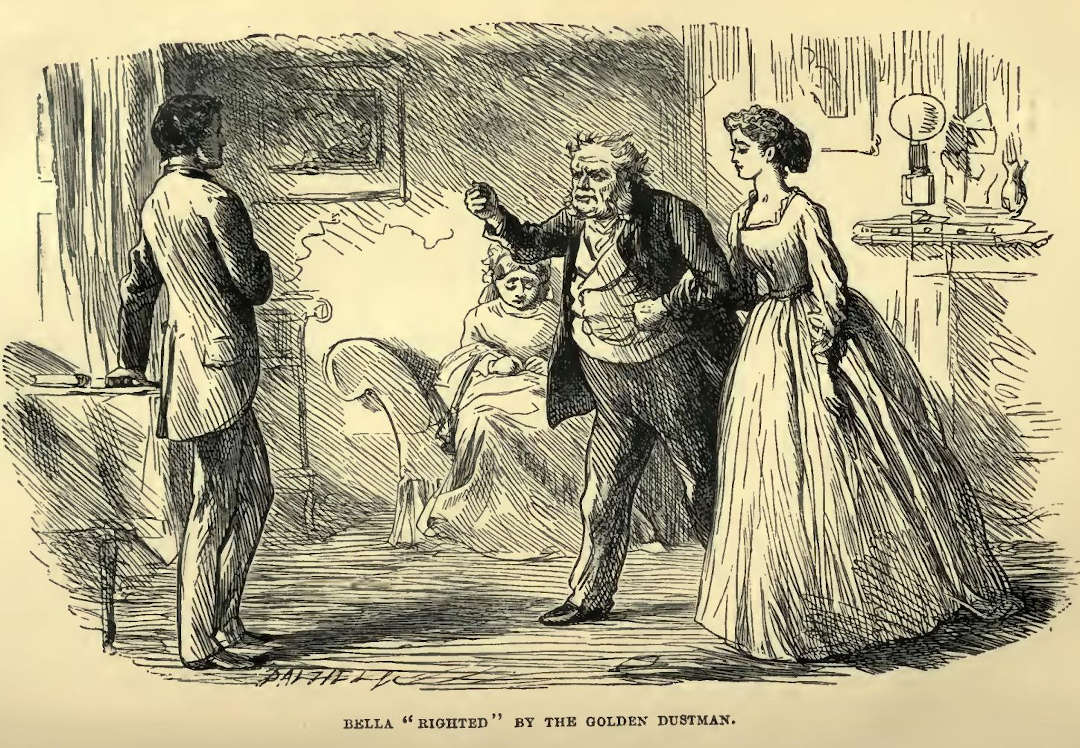
\includegraphics[scale=2.3]{03-15-01}

Bella involuntarily raising her eyes, when this sudden reference was
made to herself, met those of Mr Rokesmith. He was pale and seemed
agitated. Then her eyes passed on to Mrs Boffin’s, and she met the look
again. In a flash it enlightened her, and she began to understand what
she had done.

‘I say to you, sir,’ Mr Boffin repeated, ‘look at this young lady on my
arm.’

‘I do so,’ returned the Secretary.

As his glance rested again on Bella for a moment, she thought there was
reproach in it. But it is possible that the reproach was within herself.

‘How dare you, sir,’ said Mr Boffin, ‘tamper, unknown to me, with this
young lady? How dare you come out of your station, and your place in my
house, to pester this young lady with your impudent addresses?’

‘I must decline to answer questions,’ said the Secretary, ‘that are so
offensively asked.’

‘You decline to answer?’ retorted Mr Boffin. ‘You decline to answer,
do you? Then I’ll tell you what it is, Rokesmith; I’ll answer for you.
There are two sides to this matter, and I’ll take ‘em separately. The
first side is, sheer Insolence. That’s the first side.’

The Secretary smiled with some bitterness, as though he would have said,
‘So I see and hear.’

‘It was sheer Insolence in you, I tell you,’ said Mr Boffin, ‘even to
think of this young lady. This young lady was far above YOU. This young
lady was no match for YOU. This young lady was lying in wait (as she was
qualified to do) for money, and you had no money.’

Bella hung her head and seemed to shrink a little from Mr Boffin’s
protecting arm.

‘What are you, I should like to know,’ pursued Mr Boffin, ‘that you were
to have the audacity to follow up this young lady? This young lady was
looking about the market for a good bid; she wasn’t in it to be snapped
up by fellows that had no money to lay out; nothing to buy with.’

‘Oh, Mr Boffin! Mrs Boffin, pray say something for me!’ murmured Bella,
disengaging her arm, and covering her face with her hands.

‘Old lady,’ said Mr Boffin, anticipating his wife, ‘you hold your
tongue. Bella, my dear, don’t you let yourself be put out. I’ll right
you.’

‘But you don’t, you don’t right me!’ exclaimed Bella, with great
emphasis. ‘You wrong me, wrong me!’

‘Don’t you be put out, my dear,’ complacently retorted Mr Boffin. ‘I’ll
bring this young man to book. Now, you Rokesmith! You can’t decline
to hear, you know, as well as to answer. You hear me tell you that the
first side of your conduct was Insolence--Insolence and Presumption.
Answer me one thing, if you can. Didn’t this young lady tell you so
herself?’

‘Did I, Mr Rokesmith?’ asked Bella with her face still covered. ‘O say,
Mr Rokesmith! Did I?’

‘Don’t be distressed, Miss Wilfer; it matters very little now.’

‘Ah! You can’t deny it, though!’ said Mr Boffin, with a knowing shake of
his head.

‘But I have asked him to forgive me since,’ cried Bella; ‘and I would
ask him to forgive me now again, upon my knees, if it would spare him!’

Here Mrs Boffin broke out a-crying.

‘Old lady,’ said Mr Boffin, ‘stop that noise! Tender-hearted in you,
Miss Bella; but I mean to have it out right through with this young man,
having got him into a corner. Now, you Rokesmith. I tell you that’s one
side of your conduct--Insolence and Presumption. Now, I’m a-coming to
the other, which is much worse. This was a speculation of yours.’

‘I indignantly deny it.’

‘It’s of no use your denying it; it doesn’t signify a bit whether
you deny it or not; I’ve got a head upon my shoulders, and it ain’t a
baby’s. What!’ said Mr Boffin, gathering himself together in his most
suspicious attitude, and wrinkling his face into a very map of curves
and corners. ‘Don’t I know what grabs are made at a man with money? If
I didn’t keep my eyes open, and my pockets buttoned, shouldn’t I
be brought to the workhouse before I knew where I was? Wasn’t the
experience of Dancer, and Elwes, and Hopkins, and Blewbury Jones, and
ever so many more of ‘em, similar to mine? Didn’t everybody want to make
grabs at what they’d got, and bring ‘em to poverty and ruin? Weren’t
they forced to hide everything belonging to ‘em, for fear it should be
snatched from ‘em? Of course they was. I shall be told next that they
didn’t know human natur!’

‘They! Poor creatures,’ murmured the Secretary.

‘What do you say?’ asked Mr Boffin, snapping at him. ‘However, you
needn’t be at the trouble of repeating it, for it ain’t worth hearing,
and won’t go down with ME. I’m a-going to unfold your plan, before this
young lady; I’m a-going to show this young lady the second view of you;
and nothing you can say will stave it off. (Now, attend here, Bella, my
dear.) Rokesmith, you’re a needy chap. You’re a chap that I pick up in
the street. Are you, or ain’t you?’

‘Go on, Mr Boffin; don’t appeal to me.’

‘Not appeal to YOU,’ retorted Mr Boffin as if he hadn’t done so. ‘No,
I should hope not! Appealing to YOU, would be rather a rum course. As I
was saying, you’re a needy chap that I pick up in the street. You come
and ask me in the street to take you for a Secretary, and I take you.
Very good.’

‘Very bad,’ murmured the Secretary.

‘What do you say?’ asked Mr Boffin, snapping at him again.

He returned no answer. Mr Boffin, after eyeing him with a comical look
of discomfited curiosity, was fain to begin afresh.

‘This Rokesmith is a needy young man that I take for my Secretary out
of the open street. This Rokesmith gets acquainted with my affairs, and
gets to know that I mean to settle a sum of money on this young lady.
“Oho!” says this Rokesmith;’ here Mr Boffin clapped a finger against
his nose, and tapped it several times with a sneaking air, as embodying
Rokesmith confidentially confabulating with his own nose; ‘“This will
be a good haul; I’ll go in for this!” And so this Rokesmith, greedy and
hungering, begins a-creeping on his hands and knees towards the money.
Not so bad a speculation either: for if this young lady had had less
spirit, or had had less sense, through being at all in the romantic
line, by George he might have worked it out and made it pay! But
fortunately she was too many for him, and a pretty figure he cuts now
he is exposed. There he stands!’ said Mr Boffin, addressing Rokesmith
himself with ridiculous inconsistency. ‘Look at him!’

‘Your unfortunate suspicions, Mr Boffin--’ began the Secretary.

‘Precious unfortunate for you, I can tell you,’ said Mr Boffin.

‘--are not to be combated by any one, and I address myself to no such
hopeless task. But I will say a word upon the truth.’

‘Yah! Much you care about the truth,’ said Mr Boffin, with a snap of his
fingers.

‘Noddy! My dear love!’ expostulated his wife.

‘Old lady,’ returned Mr Boffin, ‘you keep still. I say to this Rokesmith
here, much he cares about the truth. I tell him again, much he cares
about the truth.’

‘Our connexion being at an end, Mr Boffin,’ said the Secretary, ‘it can
be of very little moment to me what you say.’

‘Oh! You are knowing enough,’ retorted Mr Boffin, with a sly look, ‘to
have found out that our connexion’s at an end, eh? But you can’t get
beforehand with me. Look at this in my hand. This is your pay, on your
discharge. You can only follow suit. You can’t deprive me of the lead.
Let’s have no pretending that you discharge yourself. I discharge you.’

‘So that I go,’ remarked the Secretary, waving the point aside with his
hand, ‘it is all one to me.’

‘Is it?’ said Mr Boffin. ‘But it’s two to me, let me tell you.
Allowing a fellow that’s found out, to discharge himself, is one thing;
discharging him for insolence and presumption, and likewise for designs
upon his master’s money, is another. One and one’s two; not one. (Old
lady, don’t you cut in. You keep still.)’

‘Have you said all you wish to say to me?’ demanded the Secretary.

‘I don’t know whether I have or not,’ answered Mr Boffin. ‘It depends.’

‘Perhaps you will consider whether there are any other strong
expressions that you would like to bestow upon me?’

‘I’ll consider that,’ said Mr Boffin, obstinately, ‘at my convenience,
and not at yours. You want the last word. It may not be suitable to let
you have it.’

‘Noddy! My dear, dear Noddy! You sound so hard!’ cried poor Mrs Boffin,
not to be quite repressed.

‘Old lady,’ said her husband, but without harshness, ‘if you cut in when
requested not, I’ll get a pillow and carry you out of the room upon it.
What do you want to say, you Rokesmith?’

‘To you, Mr Boffin, nothing. But to Miss Wilfer and to your good kind
wife, a word.’

‘Out with it then,’ replied Mr Boffin, ‘and cut it short, for we’ve had
enough of you.’

‘I have borne,’ said the Secretary, in a low voice, ‘with my false
position here, that I might not be separated from Miss Wilfer. To be
near her, has been a recompense to me from day to day, even for the
undeserved treatment I have had here, and for the degraded aspect in
which she has often seen me. Since Miss Wilfer rejected me, I have never
again urged my suit, to the best of my belief, with a spoken syllable or
a look. But I have never changed in my devotion to her, except--if she
will forgive my saying so--that it is deeper than it was, and better
founded.’

‘Now, mark this chap’s saying Miss Wilfer, when he means L.s.d.!’ cried
Mr Boffin, with a cunning wink. ‘Now, mark this chap’s making Miss
Wilfer stand for Pounds, Shillings, and Pence!’

‘My feeling for Miss Wilfer,’ pursued the Secretary, without deigning to
notice him, ‘is not one to be ashamed of. I avow it. I love her. Let
me go where I may when I presently leave this house, I shall go into a
blank life, leaving her.’

‘Leaving L.s.d. behind me,’ said Mr Boffin, by way of commentary, with
another wink.

‘That I am incapable,’ the Secretary went on, still without heeding him,
‘of a mercenary project, or a mercenary thought, in connexion with Miss
Wilfer, is nothing meritorious in me, because any prize that I could
put before my fancy would sink into insignificance beside her. If
the greatest wealth or the highest rank were hers, it would only be
important in my sight as removing her still farther from me, and making
me more hopeless, if that could be. Say,’ remarked the Secretary,
looking full at his late master, ‘say that with a word she could strip
Mr Boffin of his fortune and take possession of it, she would be of no
greater worth in my eyes than she is.’

‘What do you think by this time, old lady,’ asked Mr Boffin, turning to
his wife in a bantering tone, ‘about this Rokesmith here, and his caring
for the truth? You needn’t say what you think, my dear, because I don’t
want you to cut in, but you can think it all the same. As to taking
possession of my property, I warrant you he wouldn’t do that himself if
he could.’

‘No,’ returned the Secretary, with another full look.

‘Ha, ha, ha!’ laughed Mr Boffin. ‘There’s nothing like a good ‘un while
you ARE about it.’

‘I have been for a moment,’ said the Secretary, turning from him and
falling into his former manner, ‘diverted from the little I have to say.
My interest in Miss Wilfer began when I first saw her; even began when I
had only heard of her. It was, in fact, the cause of my throwing myself
in Mr Boffin’s way, and entering his service. Miss Wilfer has never
known this until now. I mention it now, only as a corroboration (though
I hope it may be needless) of my being free from the sordid design
attributed to me.’

‘Now, this is a very artful dog,’ said Mr Boffin, with a deep look.
‘This is a longer-headed schemer than I thought him. See how patiently
and methodically he goes to work. He gets to know about me and my
property, and about this young lady, and her share in poor young John’s
story, and he puts this and that together, and he says to himself, “I’ll
get in with Boffin, and I’ll get in with this young lady, and I’ll work
‘em both at the same time, and I’ll bring my pigs to market somewhere.”
 I hear him say it, bless you! I look at him, now, and I see him say it!’

Mr Boffin pointed at the culprit, as it were in the act, and hugged
himself in his great penetration.

‘But luckily he hadn’t to deal with the people he supposed, Bella, my
dear!’ said Mr Boffin. ‘No! Luckily he had to deal with you, and with
me, and with Daniel and Miss Dancer, and with Elwes, and with Vulture
Hopkins, and with Blewbury Jones and all the rest of us, one down
t’other come on. And he’s beat; that’s what he is; regularly beat. He
thought to squeeze money out of us, and he has done for himself instead,
Bella my dear!’

Bella my dear made no response, gave no sign of acquiescence. When she
had first covered her face she had sunk upon a chair with her hands
resting on the back of it, and had never moved since. There was a short
silence at this point, and Mrs Boffin softly rose as if to go to her.
But, Mr Boffin stopped her with a gesture, and she obediently sat down
again and stayed where she was.

‘There’s your pay, Mister Rokesmith,’ said the Golden Dustman,
jerking the folded scrap of paper he had in his hand, towards his late
Secretary. ‘I dare say you can stoop to pick it up, after what you have
stooped to here.’

‘I have stooped to nothing but this,’ Rokesmith answered as he took it
from the ground; ‘and this is mine, for I have earned it by the hardest
of hard labour.’

‘You’re a pretty quick packer, I hope,’ said Mr Boffin; ‘because the
sooner you are gone, bag and baggage, the better for all parties.’

‘You need have no fear of my lingering.’

‘There’s just one thing though,’ said Mr Boffin, ‘that I should like to
ask you before we come to a good riddance, if it was only to show this
young lady how conceited you schemers are, in thinking that nobody finds
out how you contradict yourselves.’

‘Ask me anything you wish to ask,’ returned Rokesmith, ‘but use the
expedition that you recommend.’

‘You pretend to have a mighty admiration for this young lady?’ said Mr
Boffin, laying his hand protectingly on Bella’s head without looking
down at her.

‘I do not pretend.’

‘Oh! Well. You HAVE a mighty admiration for this young lady--since you
are so particular?’

‘Yes.’

‘How do you reconcile that, with this young lady’s being a
weak-spirited, improvident idiot, not knowing what was due to herself,
flinging up her money to the church-weathercocks, and racing off at a
splitting pace for the workhouse?’

‘I don’t understand you.’

‘Don’t you? Or won’t you? What else could you have made this young lady
out to be, if she had listened to such addresses as yours?’

‘What else, if I had been so happy as to win her affections and possess
her heart?’

‘Win her affections,’ retorted Mr Boffin, with ineffable contempt,
‘and possess her heart! Mew says the cat, Quack-quack says the duck,
Bow-wow-wow says the dog! Win her affections and possess her heart! Mew,
Quack-quack, Bow-wow!’

John Rokesmith stared at him in his outburst, as if with some faint idea
that he had gone mad.

‘What is due to this young lady,’ said Mr Boffin, ‘is Money, and this
young lady right well knows it.’

‘You slander the young lady.’

‘YOU slander the young lady; you with your affections and hearts and
trumpery,’ returned Mr Boffin. ‘It’s of a piece with the rest of your
behaviour. I heard of these doings of yours only last night, or you
should have heard of ‘em from me, sooner, take your oath of it. I heard
of ‘em from a lady with as good a headpiece as the best, and she knows
this young lady, and I know this young lady, and we all three know that
it’s Money she makes a stand for--money, money, money--and that you and
your affections and hearts are a Lie, sir!’

‘Mrs Boffin,’ said Rokesmith, quietly turning to her, ‘for your delicate
and unvarying kindness I thank you with the warmest gratitude. Good-bye!
Miss Wilfer, good-bye!’

‘And now, my dear,’ said Mr Boffin, laying his hand on Bella’s head
again, ‘you may begin to make yourself quite comfortable, and I hope you
feel that you’ve been righted.’

But, Bella was so far from appearing to feel it, that she shrank from
his hand and from the chair, and, starting up in an incoherent passion
of tears, and stretching out her arms, cried, ‘O Mr Rokesmith, before
you go, if you could but make me poor again! O! Make me poor again,
Somebody, I beg and pray, or my heart will break if this goes on! Pa,
dear, make me poor again and take me home! I was bad enough there, but
I have been so much worse here. Don’t give me money, Mr Boffin, I won’t
have money. Keep it away from me, and only let me speak to good little
Pa, and lay my head upon his shoulder, and tell him all my griefs.
Nobody else can understand me, nobody else can comfort me, nobody else
knows how unworthy I am, and yet can love me like a little child. I am
better with Pa than any one--more innocent, more sorry, more glad!’ So,
crying out in a wild way that she could not bear this, Bella drooped her
head on Mrs Boffin’s ready breast.

John Rokesmith from his place in the room, and Mr Boffin from his,
looked on at her in silence until she was silent herself. Then Mr Boffin
observed in a soothing and comfortable tone, ‘There, my dear, there; you
are righted now, and it’s ALL right. I don’t wonder, I’m sure, at your
being a little flurried by having a scene with this fellow, but it’s all
over, my dear, and you’re righted, and it’s--and it’s ALL right!’ Which
Mr Boffin repeated with a highly satisfied air of completeness and
finality.

‘I hate you!’ cried Bella, turning suddenly upon him, with a stamp of
her little foot--‘at least, I can’t hate you, but I don’t like you!’

‘HUL--LO!’ exclaimed Mr Boffin in an amazed under-tone.

‘You’re a scolding, unjust, abusive, aggravating, bad old creature!’
cried Bella. ‘I am angry with my ungrateful self for calling you names;
but you are, you are; you know you are!’

Mr Boffin stared here, and stared there, as misdoubting that he must be
in some sort of fit.

‘I have heard you with shame,’ said Bella. ‘With shame for myself, and
with shame for you. You ought to be above the base tale-bearing of a
time-serving woman; but you are above nothing now.’

Mr Boffin, seeming to become convinced that this was a fit, rolled his
eyes and loosened his neckcloth.

‘When I came here, I respected you and honoured you, and I soon loved
you,’ cried Bella. ‘And now I can’t bear the sight of you. At least, I
don’t know that I ought to go so far as that--only you’re a--you’re a
Monster!’ Having shot this bolt out with a great expenditure of force,
Bella hysterically laughed and cried together.

‘The best wish I can wish you is,’ said Bella, returning to the charge,
‘that you had not one single farthing in the world. If any true friend
and well-wisher could make you a bankrupt, you would be a Duck; but as a
man of property you are a Demon!’

After despatching this second bolt with a still greater expenditure of
force, Bella laughed and cried still more.

‘Mr Rokesmith, pray stay one moment. Pray hear one word from me before
you go! I am deeply sorry for the reproaches you have borne on my
account. Out of the depths of my heart I earnestly and truly beg your
pardon.’

As she stepped towards him, he met her. As she gave him her hand, he put
it to his lips, and said, ‘God bless you!’ No laughing was mixed with
Bella’s crying then; her tears were pure and fervent.

‘There is not an ungenerous word that I have heard addressed to
you--heard with scorn and indignation, Mr Rokesmith--but it has wounded
me far more than you, for I have deserved it, and you never have. Mr
Rokesmith, it is to me you owe this perverted account of what passed
between us that night. I parted with the secret, even while I was angry
with myself for doing so. It was very bad in me, but indeed it was not
wicked. I did it in a moment of conceit and folly--one of my many such
moments--one of my many such hours--years. As I am punished for it
severely, try to forgive it!’

‘I do with all my soul.’

‘Thank you. O thank you! Don’t part from me till I have said one other
word, to do you justice. The only fault you can be truly charged with,
in having spoken to me as you did that night--with how much delicacy
and how much forbearance no one but I can know or be grateful to you
for--is, that you laid yourself open to be slighted by a worldly shallow
girl whose head was turned, and who was quite unable to rise to the
worth of what you offered her. Mr Rokesmith, that girl has often seen
herself in a pitiful and poor light since, but never in so pitiful
and poor a light as now, when the mean tone in which she answered
you--sordid and vain girl that she was--has been echoed in her ears by
Mr Boffin.’

He kissed her hand again.

‘Mr Boffin’s speeches were detestable to me, shocking to me,’ said
Bella, startling that gentleman with another stamp of her little
foot. ‘It is quite true that there was a time, and very lately, when I
deserved to be so “righted,” Mr Rokesmith; but I hope that I shall never
deserve it again!’

He once more put her hand to his lips, and then relinquished it, and
left the room. Bella was hurrying back to the chair in which she had
hidden her face so long, when, catching sight of Mrs Boffin by the
way, she stopped at her. ‘He is gone,’ sobbed Bella indignantly,
despairingly, in fifty ways at once, with her arms round Mrs Boffin’s
neck. ‘He has been most shamefully abused, and most unjustly and most
basely driven away, and I am the cause of it!’

All this time, Mr Boffin had been rolling his eyes over his loosened
neckerchief, as if his fit were still upon him. Appearing now to think
that he was coming to, he stared straight before him for a while, tied
his neckerchief again, took several long inspirations, swallowed several
times, and ultimately exclaimed with a deep sigh, as if he felt himself
on the whole better: ‘Well!’

No word, good or bad, did Mrs Boffin say; but she tenderly took care of
Bella, and glanced at her husband as if for orders. Mr Boffin, without
imparting any, took his seat on a chair over against them, and there
sat leaning forward, with a fixed countenance, his legs apart, a hand on
each knee, and his elbows squared, until Bella should dry her eyes and
raise her head, which in the fulness of time she did.

‘I must go home,’ said Bella, rising hurriedly. ‘I am very grateful to
you for all you have done for me, but I can’t stay here.’

‘My darling girl!’ remonstrated Mrs Boffin.

‘No, I can’t stay here,’ said Bella; ‘I can’t indeed.--Ugh! you vicious
old thing!’ (This to Mr Boffin.)

‘Don’t be rash, my love,’ urged Mrs Boffin. ‘Think well of what you do.’

‘Yes, you had better think well,’ said Mr Boffin.

‘I shall never more think well of YOU,’ cried Bella, cutting him
short, with intense defiance in her expressive little eyebrows, and
championship of the late Secretary in every dimple. ‘No! Never again!
Your money has changed you to marble. You are a hard-hearted Miser. You
are worse than Dancer, worse than Hopkins, worse than Blackberry Jones,
worse than any of the wretches. And more!’ proceeded Bella, breaking
into tears again, ‘you were wholly undeserving of the Gentleman you have
lost.’

‘Why, you don’t mean to say, Miss Bella,’ the Golden Dustman slowly
remonstrated, ‘that you set up Rokesmith against me?’

‘I do!’ said Bella. ‘He is worth a Million of you.’

Very pretty she looked, though very angry, as she made herself as
tall as she possibly could (which was not extremely tall), and utterly
renounced her patron with a lofty toss of her rich brown head.

‘I would rather he thought well of me,’ said Bella, ‘though he swept the
street for bread, than that you did, though you splashed the mud upon
him from the wheels of a chariot of pure gold.--There!’

‘Well I’m sure!’ cried Mr Boffin, staring.

‘And for a long time past, when you have thought you set yourself above
him, I have only seen you under his feet,’ said Bella--‘There! And
throughout I saw in him the master, and I saw in you the man--There! And
when you used him shamefully, I took his part and loved him--There! I
boast of it!’

After which strong avowal Bella underwent reaction, and cried to any
extent, with her face on the back of her chair.

‘Now, look here,’ said Mr Boffin, as soon as he could find an opening
for breaking the silence and striking in. ‘Give me your attention,
Bella. I am not angry.’

‘I AM!’ said Bella.

‘I say,’ resumed the Golden Dustman, ‘I am not angry, and I mean kindly
to you, and I want to overlook this. So you’ll stay where you are, and
we’ll agree to say no more about it.’

‘No, I can’t stay here,’ cried Bella, rising hurriedly again; ‘I can’t
think of staying here. I must go home for good.’

‘Now, don’t be silly,’ Mr Boffin reasoned. ‘Don’t do what you can’t
undo; don’t do what you’re sure to be sorry for.’

‘I shall never be sorry for it,’ said Bella; ‘and I should always be
sorry, and should every minute of my life despise myself if I remained
here after what has happened.’

‘At least, Bella,’ argued Mr Boffin, ‘let there be no mistake about it.
Look before you leap, you know. Stay where you are, and all’s well, and
all’s as it was to be. Go away, and you can never come back.’

‘I know that I can never come back, and that’s what I mean,’ said Bella.

‘You mustn’t expect,’ Mr Boffin pursued, ‘that I’m a-going to settle
money on you, if you leave us like this, because I am not. No, Bella! Be
careful! Not one brass farthing.’

‘Expect!’ said Bella, haughtily. ‘Do you think that any power on earth
could make me take it, if you did, sir?’

But there was Mrs Boffin to part from, and, in the full flush of her
dignity, the impressible little soul collapsed again. Down upon her
knees before that good woman, she rocked herself upon her breast, and
cried, and sobbed, and folded her in her arms with all her might.

‘You’re a dear, a dear, the best of dears!’ cried Bella. ‘You’re the
best of human creatures. I can never be thankful enough to you, and I
can never forget you. If I should live to be blind and deaf I know I
shall see and hear you, in my fancy, to the last of my dim old days!’

Mrs Boffin wept most heartily, and embraced her with all fondness; but
said not one single word except that she was her dear girl. She said
that often enough, to be sure, for she said it over and over again; but
not one word else.

Bella broke from her at length, and was going weeping out of the room,
when in her own little queer affectionate way, she half relented towards
Mr Boffin.

‘I am very glad,’ sobbed Bella, ‘that I called you names, sir, because
you richly deserved it. But I am very sorry that I called you names,
because you used to be so different. Say good-bye!’

‘Good-bye,’ said Mr Boffin, shortly.

‘If I knew which of your hands was the least spoilt, I would ask you
to let me touch it,’ said Bella, ‘for the last time. But not because I
repent of what I have said to you. For I don’t. It’s true!’

‘Try the left hand,’ said Mr Boffin, holding it out in a stolid manner;
‘it’s the least used.’

‘You have been wonderfully good and kind to me,’ said Bella, ‘and I kiss
it for that. You have been as bad as bad could be to Mr Rokesmith, and I
throw it away for that. Thank you for myself, and good-bye!’

‘Good-bye,’ said Mr Boffin as before.

Bella caught him round the neck and kissed him, and ran out for ever.

She ran up-stairs, and sat down on the floor in her own room, and cried
abundantly. But the day was declining and she had no time to lose. She
opened all the places where she kept her dresses; selected only those
she had brought with her, leaving all the rest; and made a great
misshapen bundle of them, to be sent for afterwards.

‘I won’t take one of the others,’ said Bella, tying the knots of the
bundle very tight, in the severity of her resolution. ‘I’ll leave all
the presents behind, and begin again entirely on my own account.’ That
the resolution might be thoroughly carried into practice, she even
changed the dress she wore, for that in which she had come to the grand
mansion. Even the bonnet she put on, was the bonnet that had mounted
into the Boffin chariot at Holloway.

‘Now, I am complete,’ said Bella. ‘It’s a little trying, but I have
steeped my eyes in cold water, and I won’t cry any more. You have been
a pleasant room to me, dear room. Adieu! We shall never see each other
again.’

With a parting kiss of her fingers to it, she softly closed the door and
went with a light foot down the great staircase, pausing and listening
as she went, that she might meet none of the household. No one chanced
to be about, and she got down to the hall in quiet. The door of the late
Secretary’s room stood open. She peeped in as she passed, and divined
from the emptiness of his table, and the general appearance of things,
that he was already gone. Softly opening the great hall door, and
softly closing it upon herself, she turned and kissed it on the
outside--insensible old combination of wood and iron that it
was!--before she ran away from the house at a swift pace.

‘That was well done!’ panted Bella, slackening in the next street, and
subsiding into a walk. ‘If I had left myself any breath to cry with, I
should have cried again. Now poor dear darling little Pa, you are going
to see your lovely woman unexpectedly.’



